\documentclass{beamer}
\useoutertheme[progressbar=frametitle]{metropolis}
\useinnertheme{metropolis}
\definecolor{nabgray}{rgb}{0.6,0.59,0.61}
\usecolortheme[named=nabgray]{structure}

\usepackage{tikz}
\usepackage[utf8]{inputenc}
\usepackage[english]{babel}

\usepackage{smartdiagram}
\usepackage{qtree}
\usepackage{verbatim}
\usepackage{svg}
\usepackage{graphicx}
\usepackage{color}
\definecolor{lightgray}{rgb}{0.95, 0.95, 0.95}
\definecolor{darkgray}{rgb}{0.4, 0.4, 0.4}
%\definecolor{purple}{rgb}{0.65, 0.12, 0.82}
\definecolor{editorGray}{rgb}{0.95, 0.95, 0.95}
\definecolor{editorOcher}{rgb}{1, 0.5, 0} % #FF7F00 -> rgb(239, 169, 0)
\definecolor{editorGreen}{rgb}{0, 0.5, 0} % #007C00 -> rgb(0, 124, 0)
\definecolor{orange}{rgb}{1,0.45,0.13}		
\definecolor{olive}{rgb}{0.17,0.59,0.20}
\definecolor{brown}{rgb}{0.69,0.31,0.31}
\definecolor{purple}{rgb}{0.38,0.18,0.81}
\definecolor{lightblue}{rgb}{0.1,0.57,0.7}
\definecolor{lightred}{rgb}{1,0.4,0.5}
\usepackage{upquote}
\usepackage{listings}
\lstset{language=java,
	basicstyle=\footnotesize\ttfamily,
	keywordstyle=\footnotesize\color{blue}\ttfamily,
}


\usebackgroundtemplate%
{%
	
\includegraphics[width=\paperwidth]{Images/Contenido}%
}


\title{Microservicios con Jakarta EE y Eclipse MicroProfile}
\author{Víctor Orozco - @tuxtor}
\institute{GuateJUG}
\date{\today}

\begin{document}

\frame{\titlepage}

\begin{frame}{Víctor Orozco}
\begin{columns}[T] % contents are top vertically aligned
	\begin{column}[T]{5cm} % each column can also be its own environment
		\begin{itemize}
			\item Developer (JVM/Open Source Advocate)
			\item JUG Leader
			\item Oracle Certified, Lightbend Certified
			\item \href{https://twitter.com/tuxtor}{@tuxtor}
			\item \href{http://vorozco.com}{http://vorozco.com}
			\item \href{http://tuxtor.shekalug.org}{http://tuxtor.shekalug.org} 
		\end{itemize}
	\end{column}
	\begin{column}[T]{5cm} % alternative top-align that's better for graphics
		\begin{figure}
			\centering
			
\includegraphics[width=0.6\linewidth]{Images/logos}
		\end{figure}
		
	\end{column}
\end{columns}
\end{frame}


%\begin{frame}{Zen State}
%Zen State of software projects

%\begin{figure}
%	\centering
%	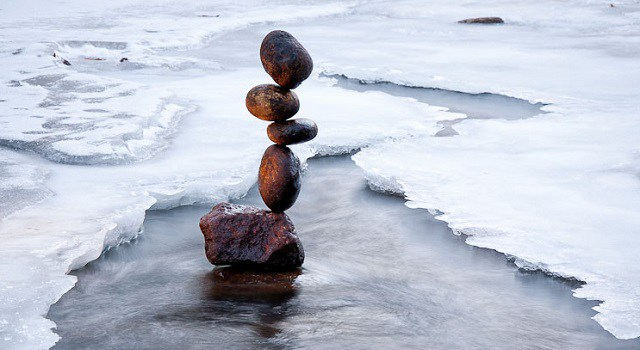
\includegraphics[width=0.7\linewidth]{Images/zen}
%\end{figure}
%\end{frame}


\section{Java EE 7}

\begin{frame}{Java EE 7}
\begin{figure}
\centering
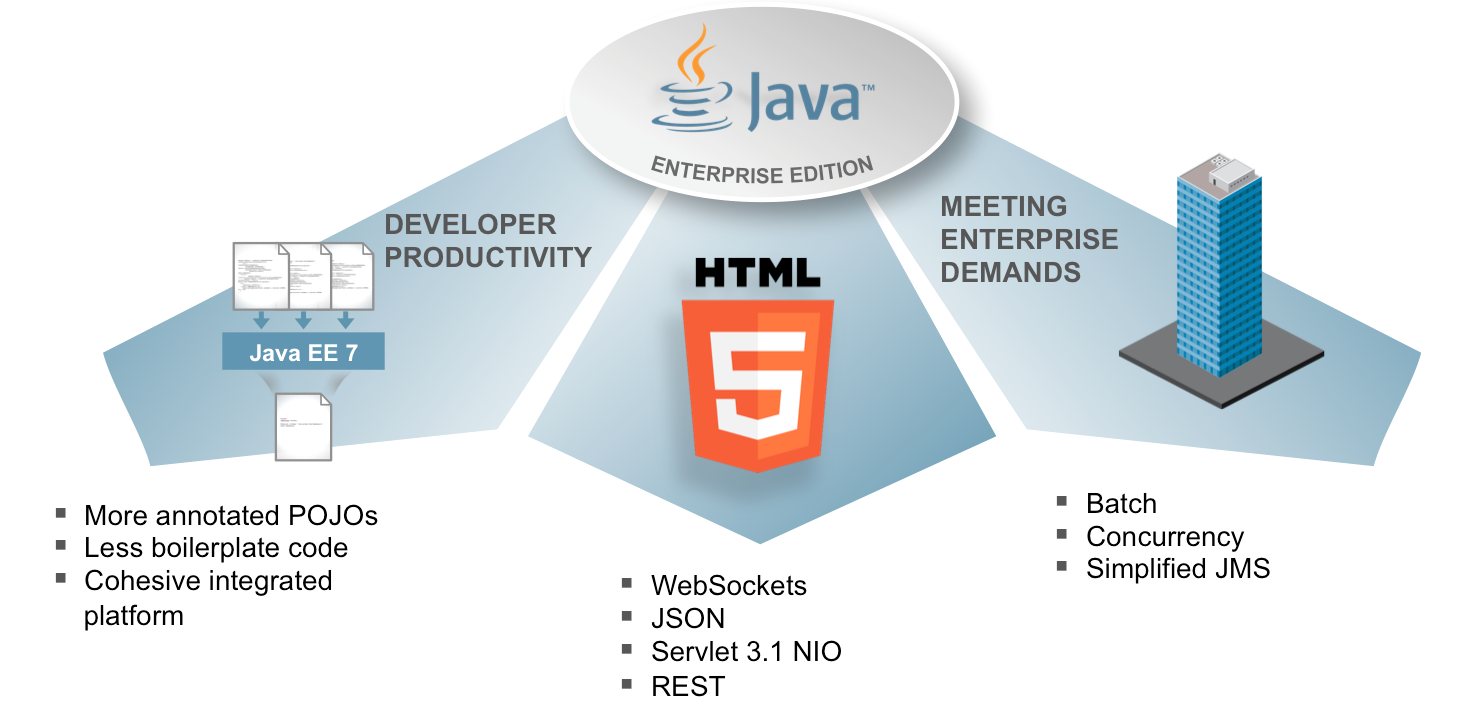
\includegraphics[width=\linewidth]{Images/javaee7-theme}
\end{figure}
\end{frame}

\begin{frame}{Java EE 7}
\begin{exampleblock}{Java EE 7}
\begin{itemize}
\item Nuevo JMS
\item WebSockets
\item JSON Support
\item Concurrency
\item Nuevo JAX-RS
\item Batch apps
\end{itemize}
\end{exampleblock}
\end{frame}



\section{Java EE 7 - La rebelión de los Dukes}

\begin{frame}{Java EE 7 - La rebelión}
\begin{columns}
\begin{column}{0.5\textwidth}
\begin{figure}
\centering

\includegraphics[width=\linewidth]{Images/microprofile-logo}
\end{figure}
\end{column}
\begin{column}{0.5\textwidth}  %%<--- here
\begin{figure}
\centering

\includegraphics[width=\linewidth]{Images/guardians}
\end{figure}
\end{column}
\end{columns}
\end{frame}


\section{Java EE 8}
\begin{frame}{Java EE 8}
\begin{figure}
	\centering
	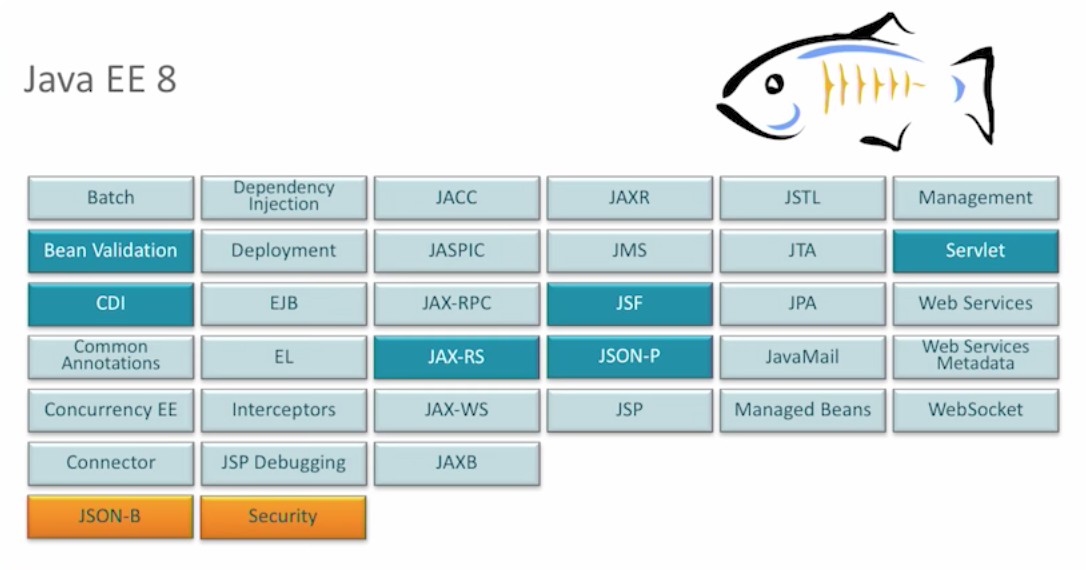
\includegraphics[width=\linewidth]{Images/javaee8}
\end{figure}
\end{frame}


\begin{frame}{Java EE 8}
\begin{alertblock}{Java EE 8}
\begin{itemize}
	\item Mejor integración de JSF con CDI
	\item Mejor integración de JMS con CDI
	\item HTTP/2
	\item JSON-B
	\item Security
	\item \textbf{JAX-RS Reactivo}
\end{itemize}
\end{alertblock}
\end{frame}

\begin{frame}{Java EE 8}
\begin{figure}
	\centering
	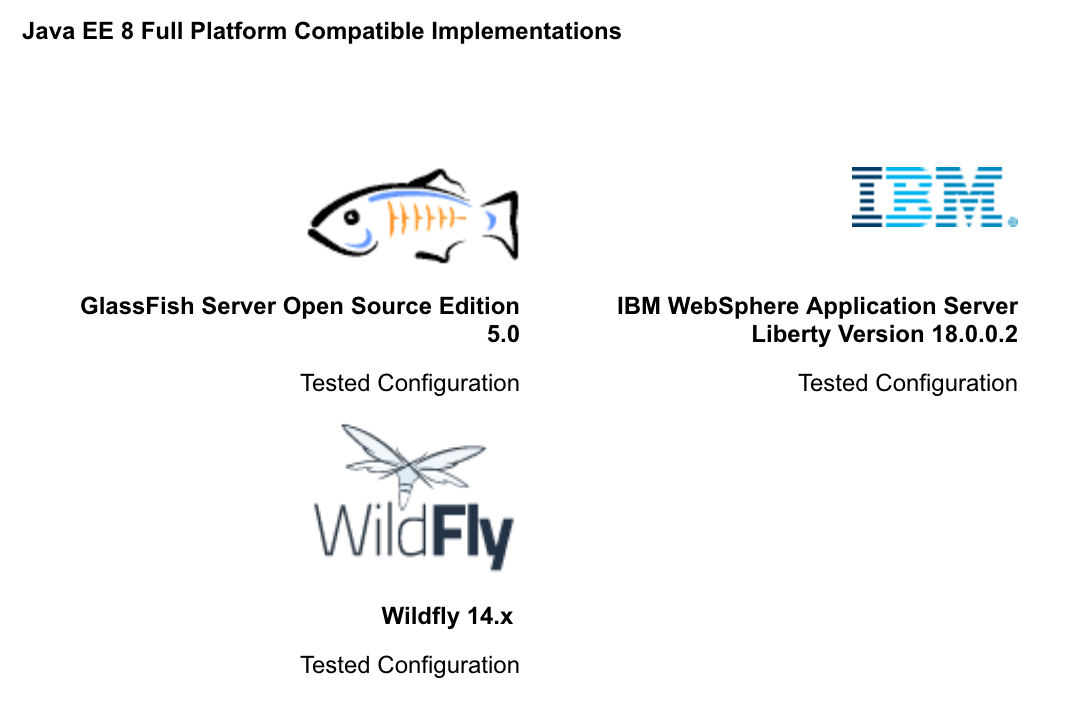
\includegraphics[width=0.7\linewidth]{Images/ee8}
\end{figure}
\end{frame}


\begin{frame}{Eclipse Jakarta EE}
\begin{figure}
	\centering
	
\includegraphics[width=0.7\linewidth]{Images/jakartaee}
\end{figure}
\end{frame}

\section{El mundo micro y sus lecciones}

\section{Lección 0: Lo que la gente realmente quiere no son microservicios, son sistemas reactivos}
\begin{frame}{Reactive Manifesto}
\begin{figure}
	\centering
	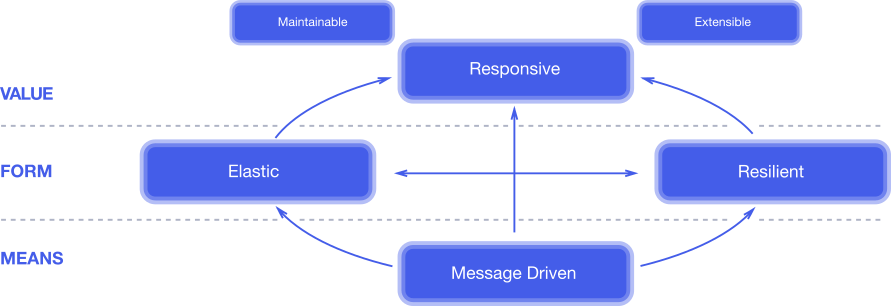
\includegraphics[width=0.9\linewidth]{Images/reactive-traits}
	\caption{https://www.reactivemanifesto.org/}
\end{figure}
\end{frame}

\begin{frame}{Microservicios}
Ventajas
\begin{itemize}
\item Bases de código pequeñas
\item Buenas practicas
\item Tolerancia a fallas
\item Escalabilidad
\end{itemize}
Desventajas
\begin{itemize}
\item Tooling overhead
\item Depuración
\item Transacciones distribuidas
\item Latencia
\item Dependencia
\end{itemize}
\end{frame}


\begin{frame}{Microservicios}
Desventaja principal \\

\huge Hype Driven Development
\end{frame}

\section{Lección 1: Los microservicios son una revolución de pensamiento}
\begin{frame}{Monolito}
\begin{figure}
	\centering
	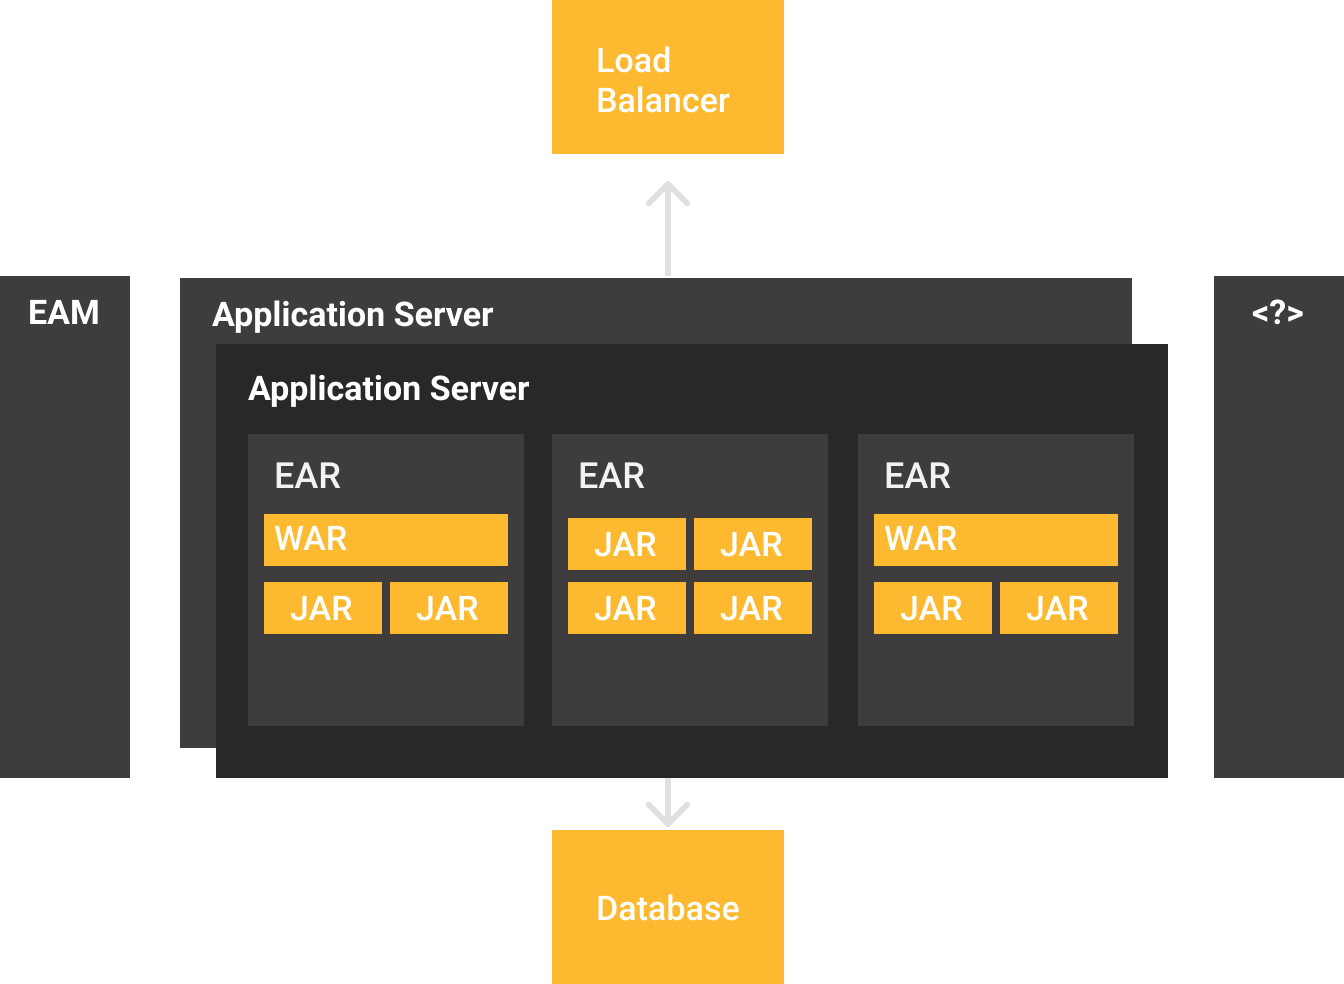
\includegraphics[width=0.7\linewidth]{Images/monolitos}
	\caption{Monolito regular}
\end{figure}
\end{frame}

\begin{frame}{ESB}
\begin{figure}
\centering
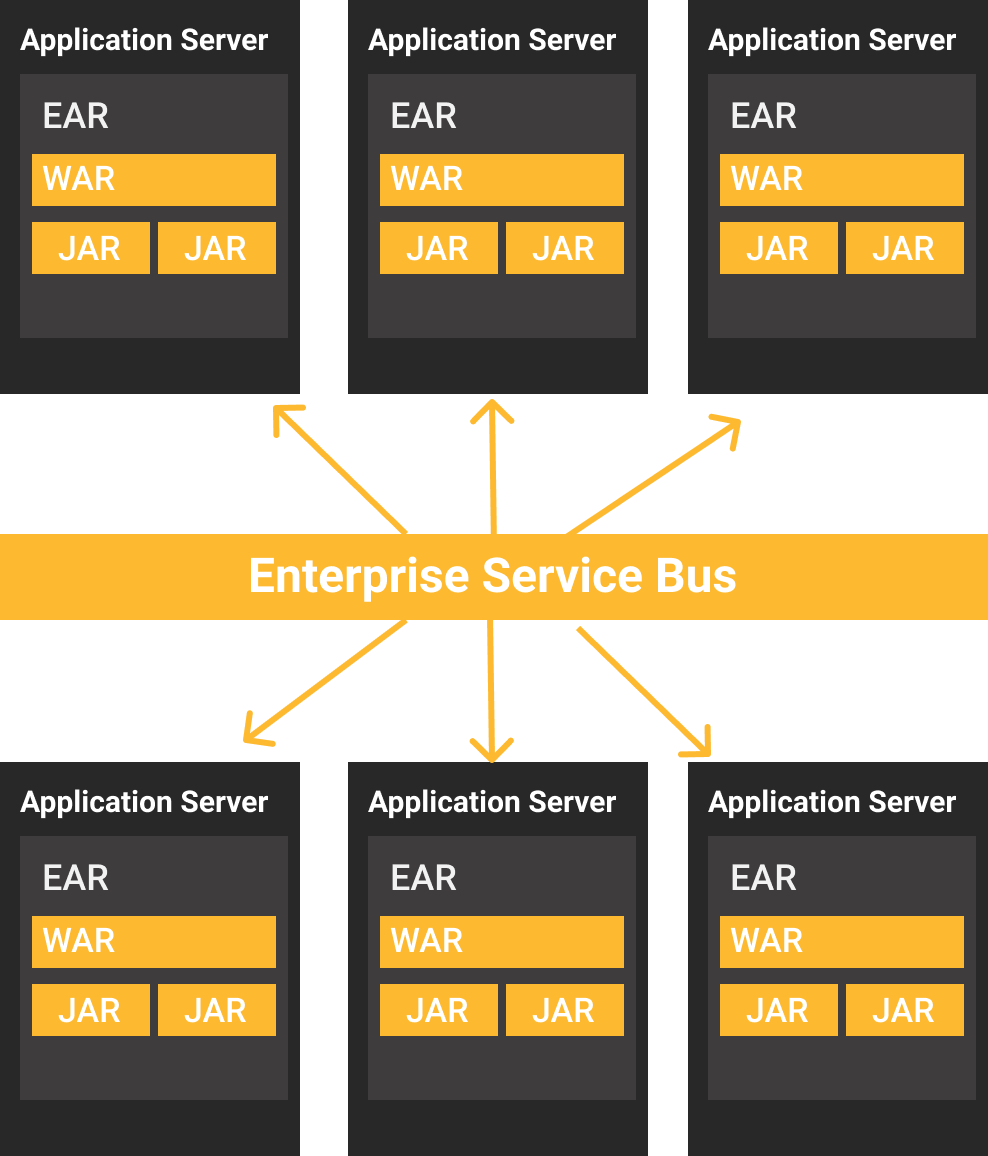
\includegraphics[width=0.5\linewidth]{Images/esb}
\caption{ESB}
\end{figure}
\end{frame}

\begin{frame}{Microservicios}
\begin{figure}
\centering
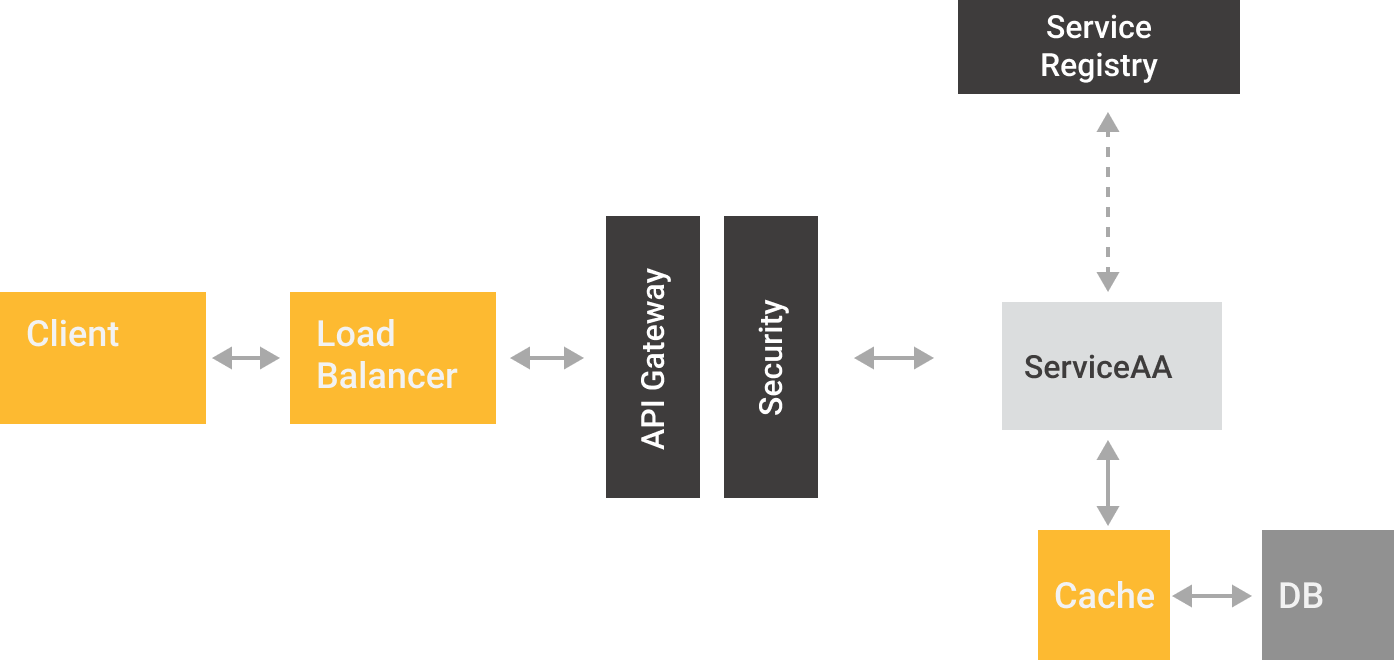
\includegraphics[width=\linewidth]{Images/microservicios}
\caption{Microservicios}
\end{figure}
\end{frame}


\section{Lección 2: Microservicios no son lo mismo para todos}
\begin{frame}{Como}
Pruebas de concepto de Sr. a Jr.
\begin{itemize}
\item Vert.x
\item Spring Boot
\item DropWizard
\item Akka
\item NodeJS
. . .
\item Java EE
\end{itemize}
\end{frame}

\begin{frame}{J2EE}
Trabajos J2EE Guatemala 2018
\begin{figure}
\centering

\includegraphics[width=\linewidth]{Images/javaee}
\end{figure}
\end{frame}

\begin{frame}{Recursos humanos}
\begin{itemize}
\item De las universidades "top" en Guatemala solo 3 enseñan Java realmente bien
\item Las otras dos enseñan .NET
\item Las Sillicon Valley off-shores se llevan a los mejores devs
\end{itemize}
\end{frame}


\section{Lección 3: No es necesario ser 100\% "microservicios"}
\begin{frame}{Microservicios - Java EE}
Java EE es el framework más anti-hype \\

\huge J2EE 1.2 (Diciembre 12, 1999)
\end{frame}


\begin{frame}{Microservicios - Java EE}
Implementación
\begin{itemize}
\item Refactoring iterativo - Por oleadas
\item Refactoring practico - Extraer solo los servicios necesarios
\item Nuevos servicios - Nuevos servicios le hablan a monolitos
\end{itemize}
\end{frame}


\begin{frame}{Microservicios - Java EE}

\begin{figure}
\centering
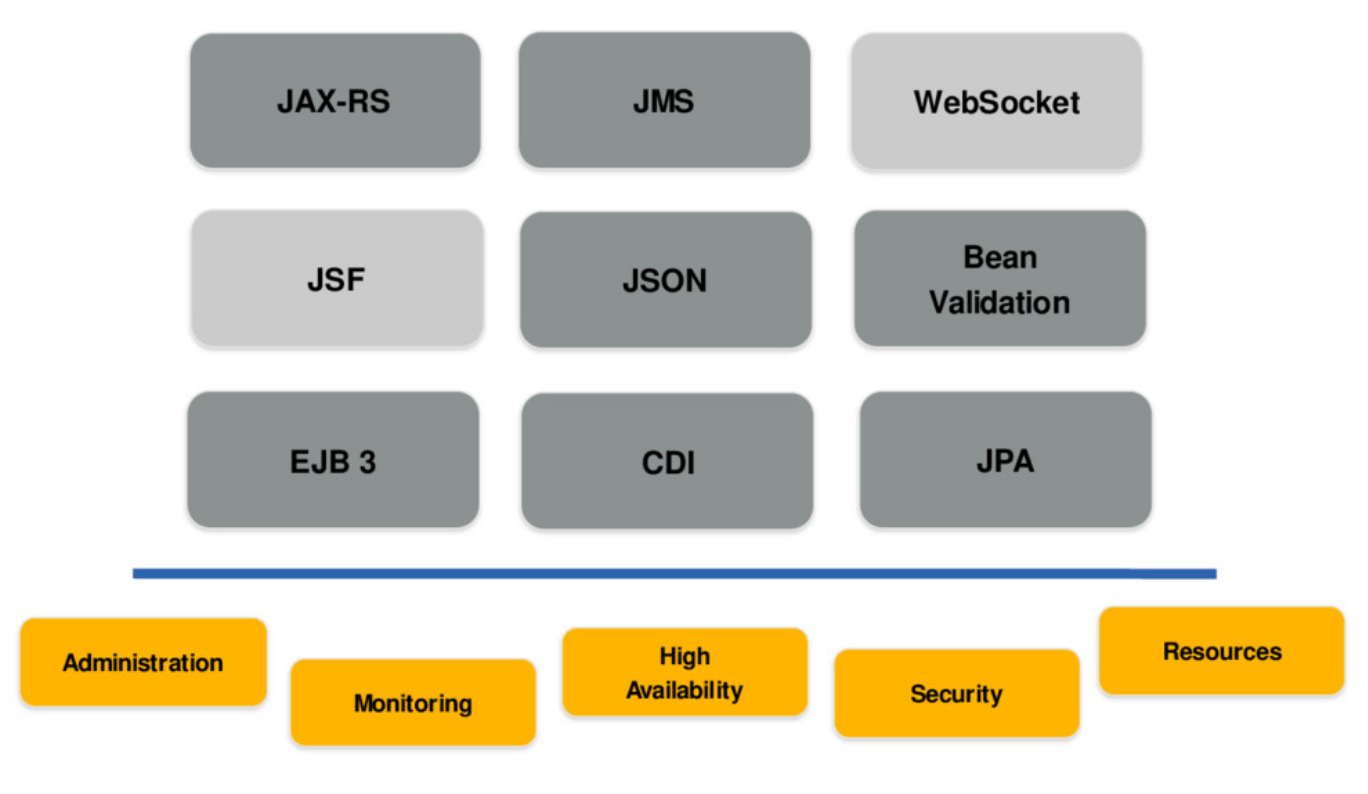
\includegraphics[width=0.9\linewidth]{Images/javaeemicropancake.png}
\caption{Tecnologías Java EE - Créditos: Reza Rahman}
\end{figure}
\end{frame}

\begin{frame}{Microservicios - Java EE}
\begin{figure}
\centering
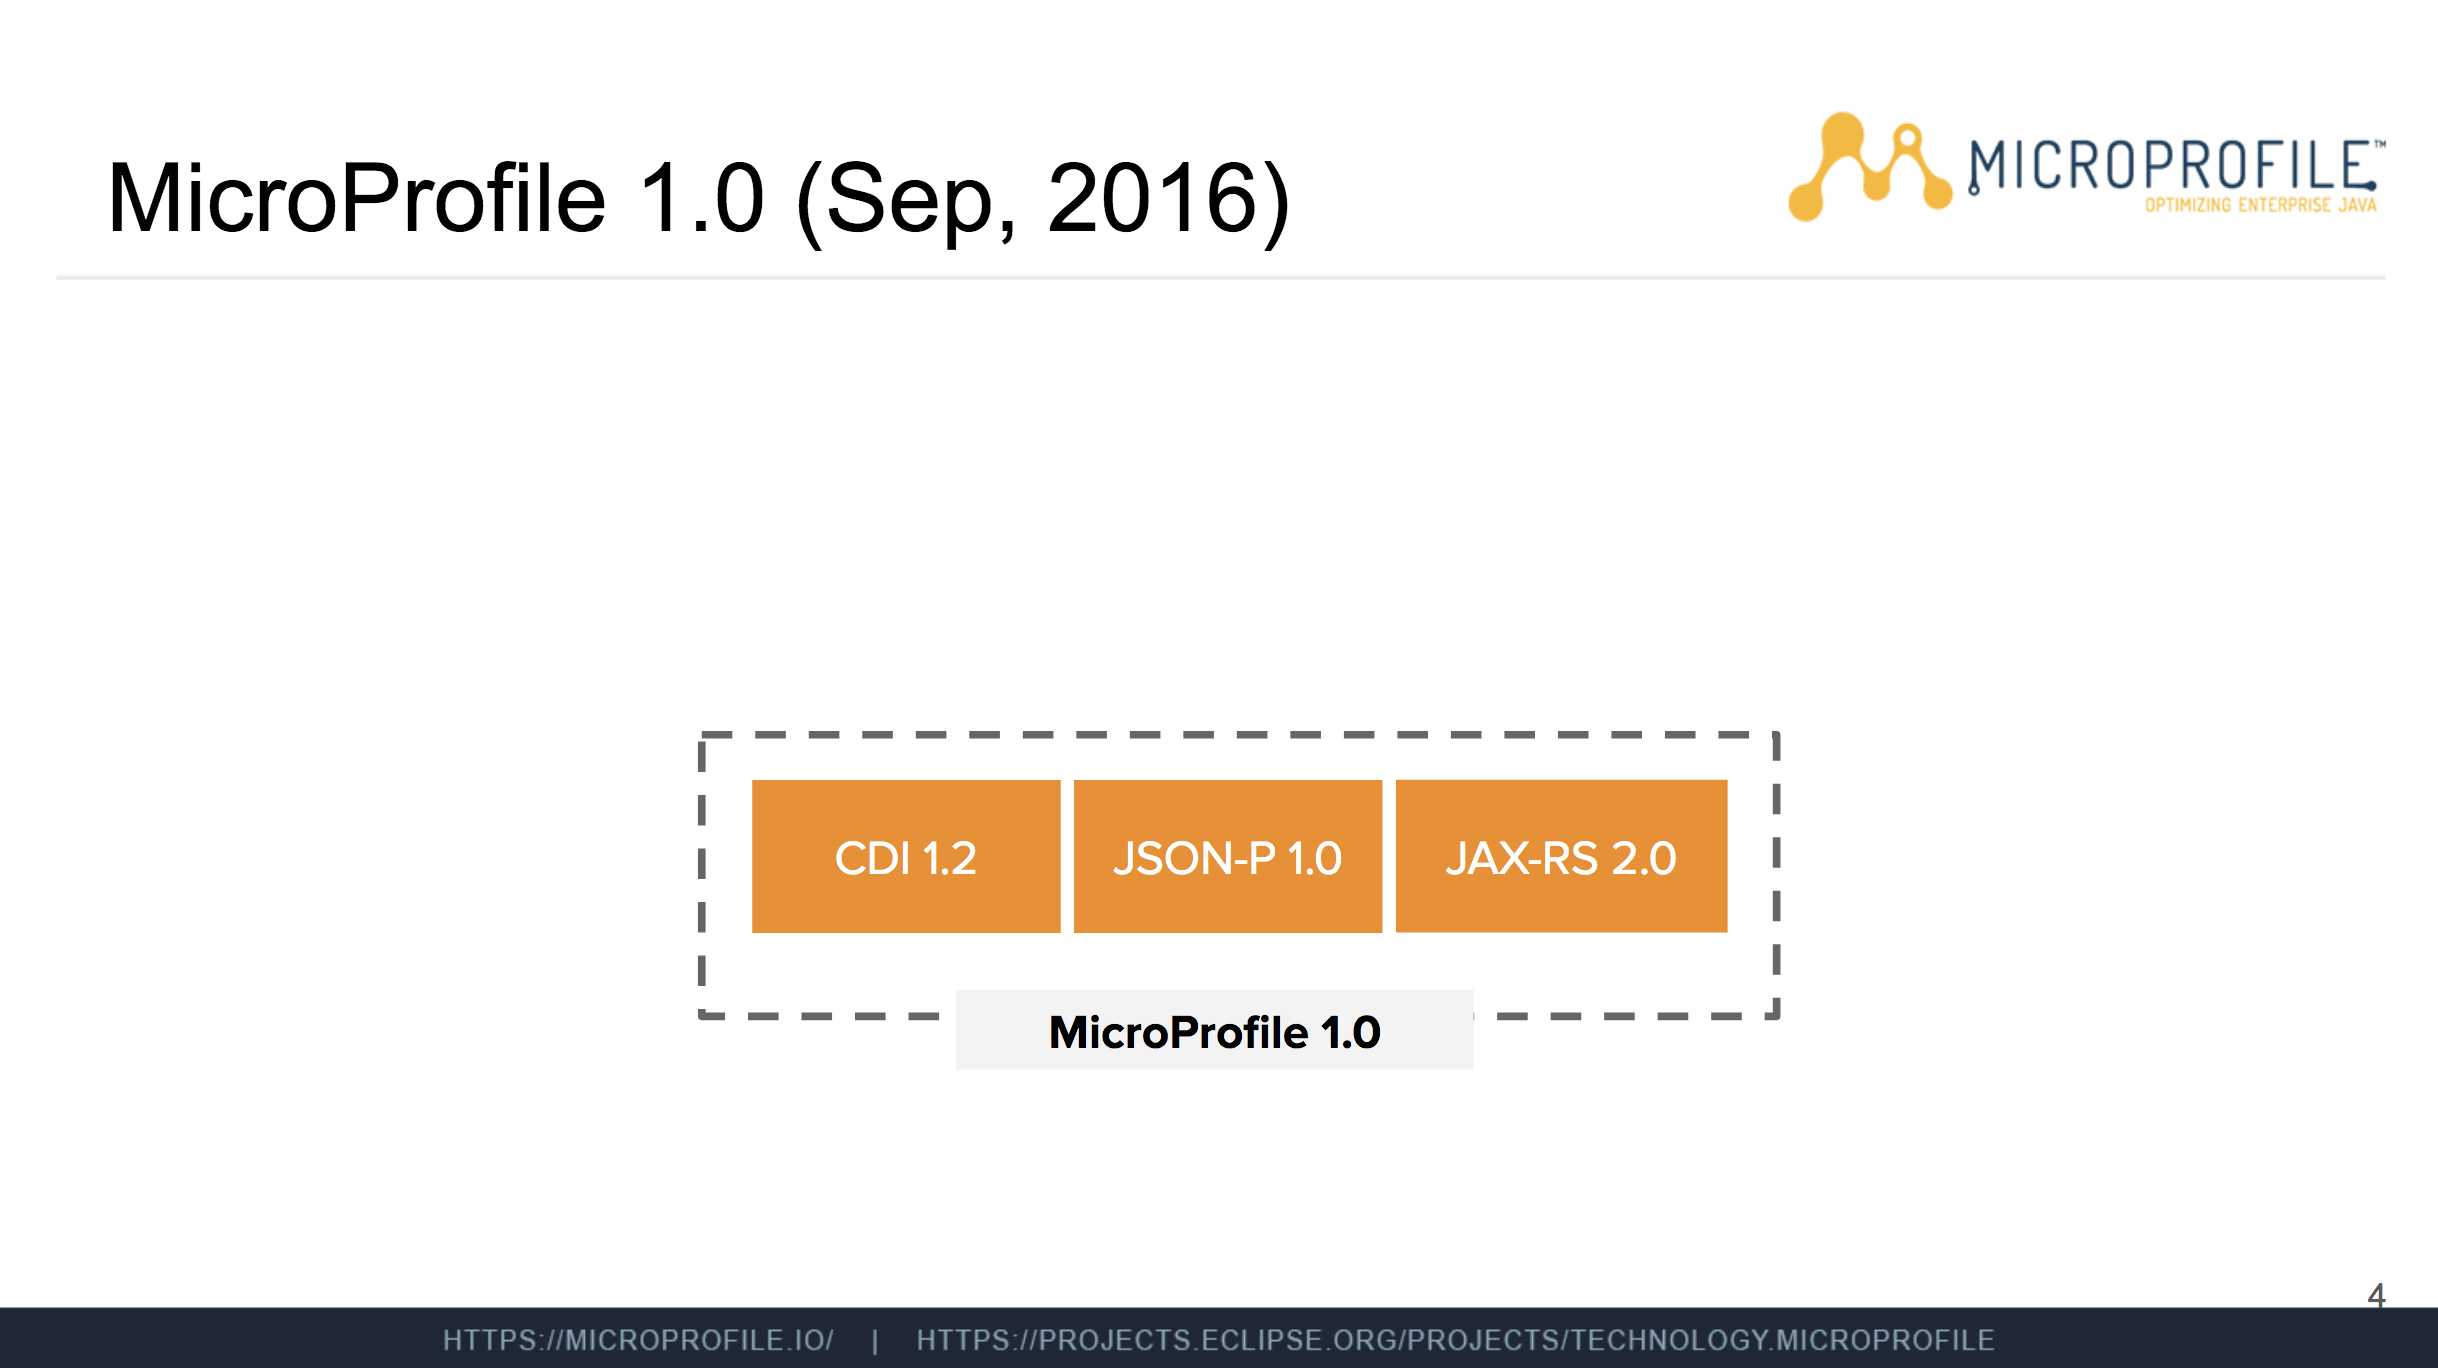
\includegraphics[width=\linewidth]{Images/mp1}
\end{figure}
\end{frame}

\begin{frame}{Microservicios - Java EE}
\begin{figure}
\centering
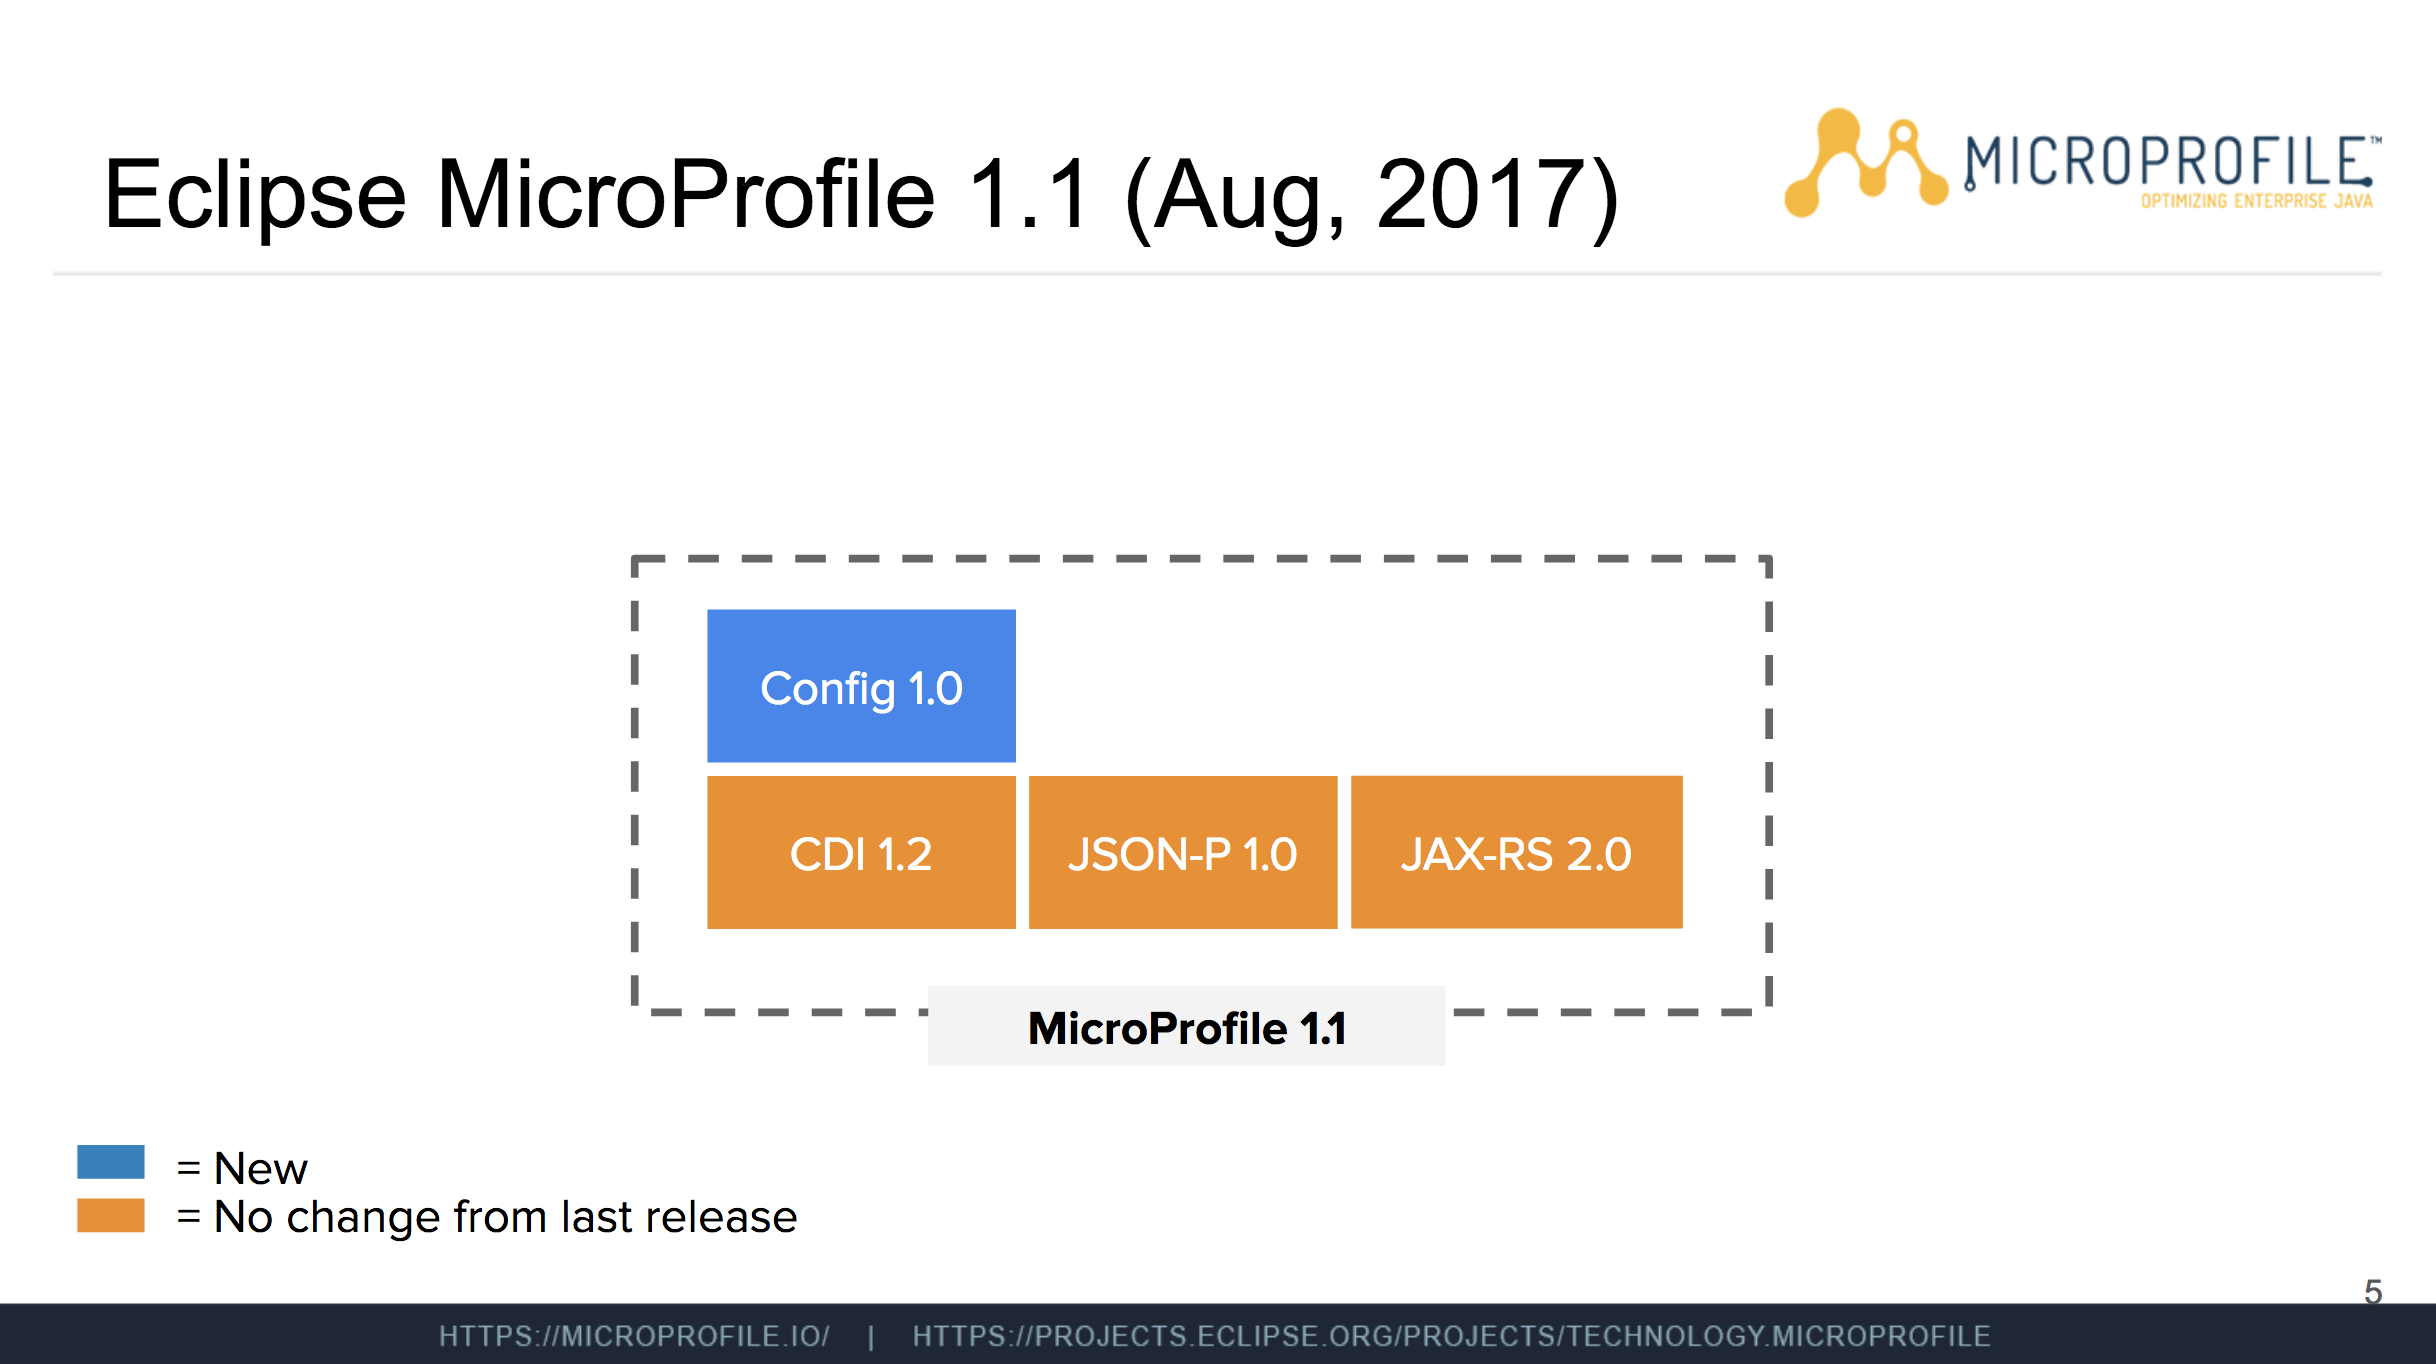
\includegraphics[width=\linewidth]{Images/mp2}
\end{figure}
\end{frame}

\begin{frame}{Microservicios - Java EE}
\begin{figure}
\centering
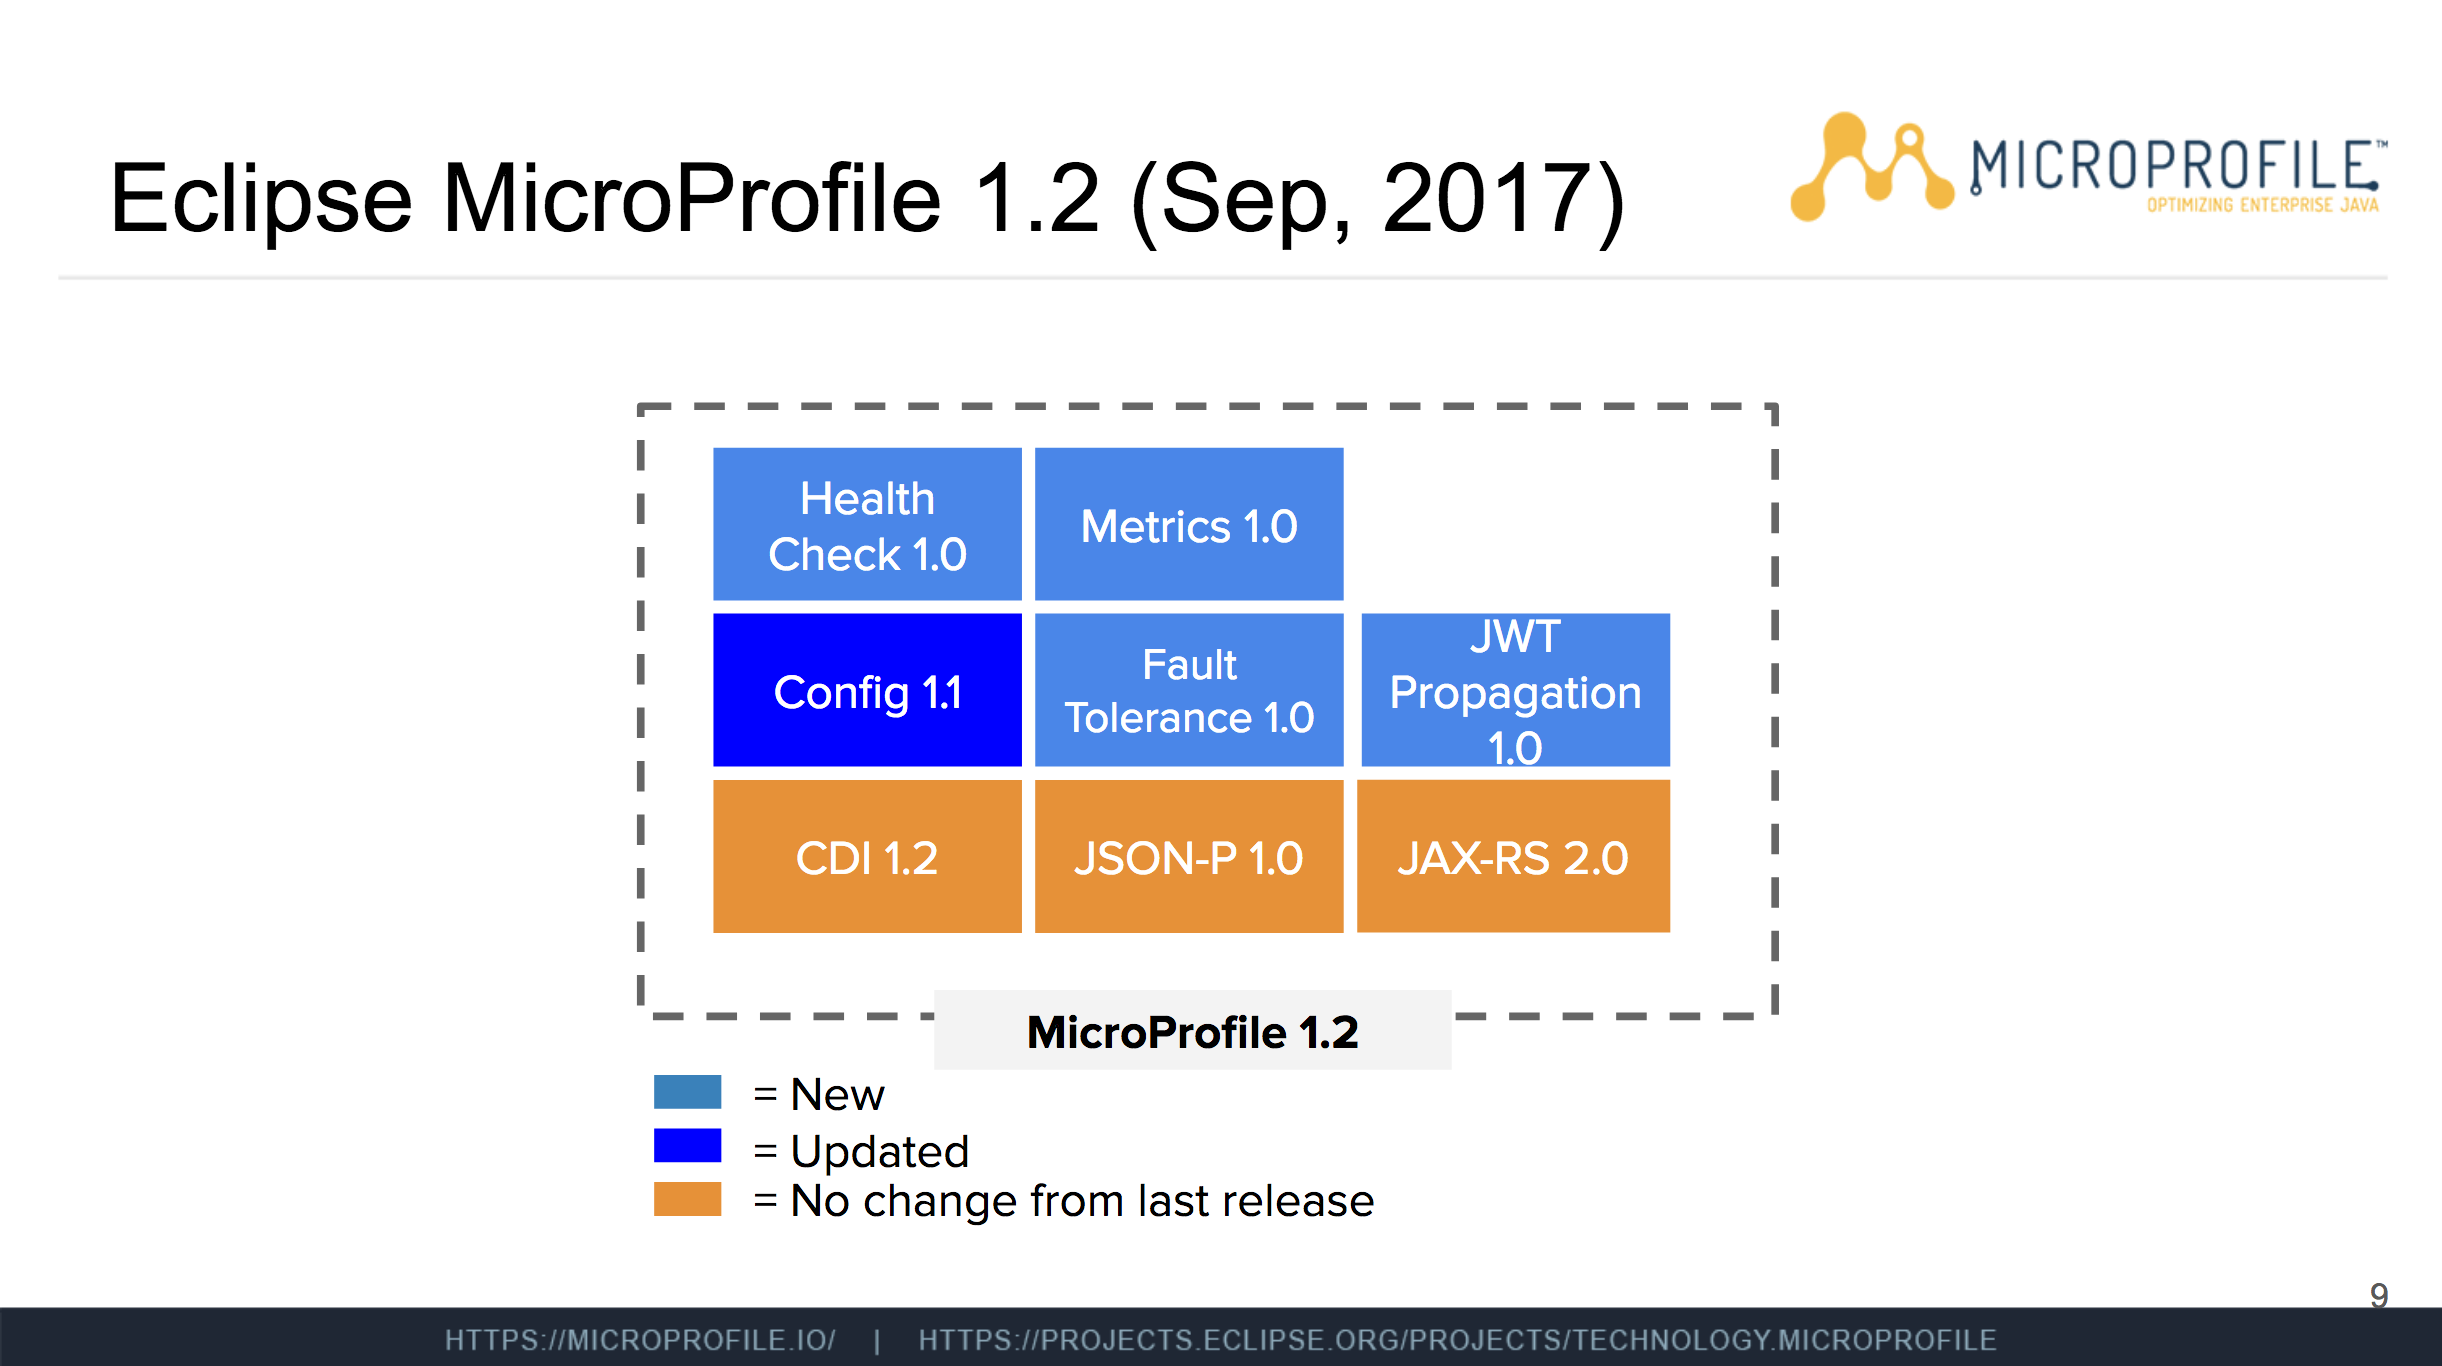
\includegraphics[width=\linewidth]{Images/mp3}
\end{figure}
\end{frame}

\begin{frame}{Microservicios - Java EE}
\begin{figure}
	\centering
	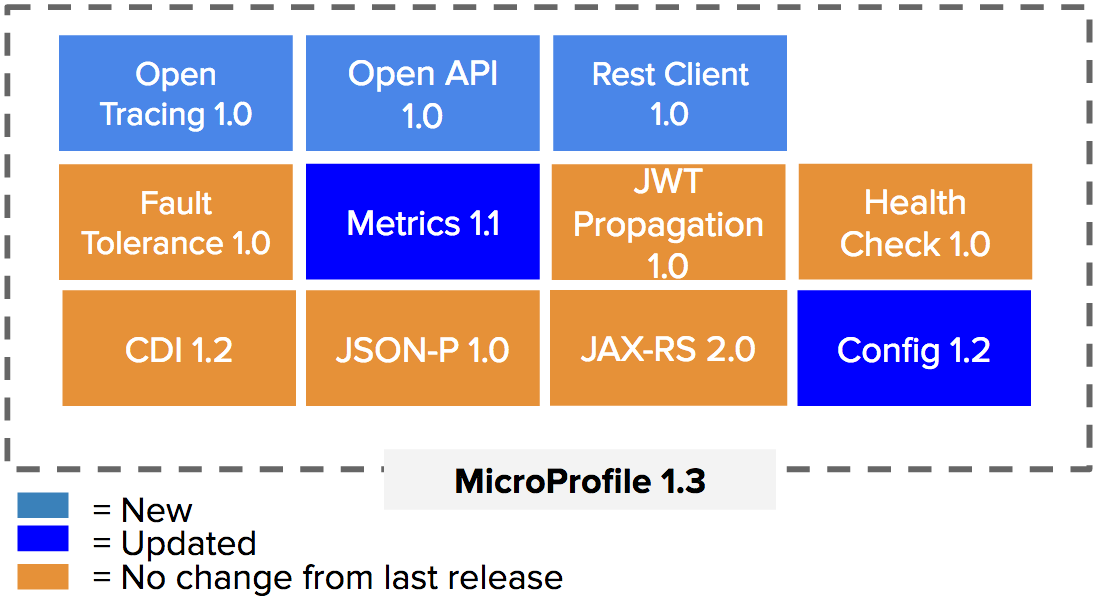
\includegraphics[width=\linewidth]{Images/mp4}
\end{figure}
\end{frame}

\begin{frame}{Microservicios - Java EE}
\begin{figure}
	\centering
	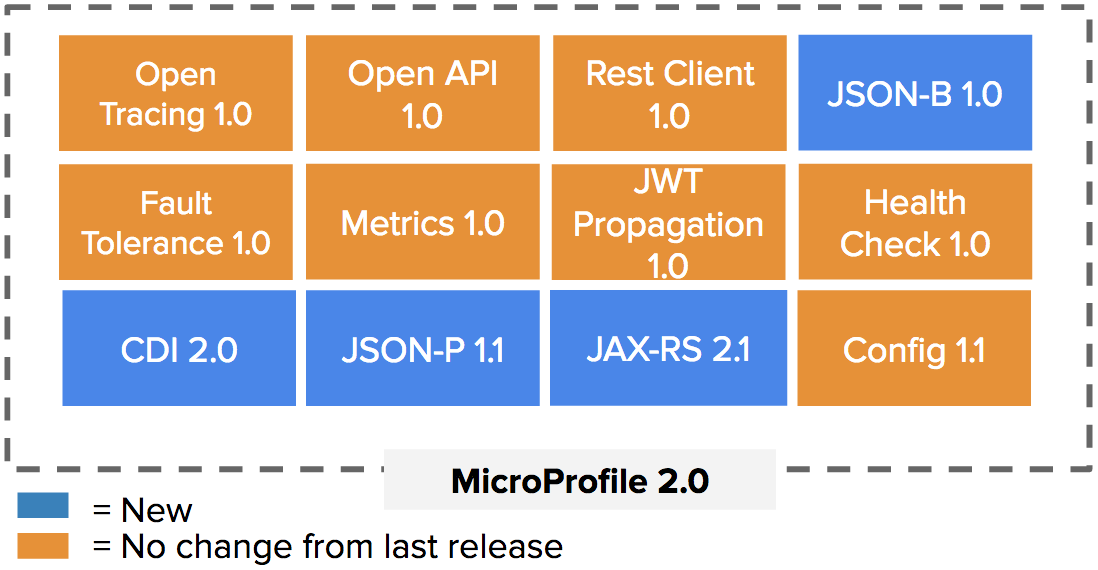
\includegraphics[width=\linewidth]{Images/mp5}
\end{figure}
\end{frame}

\begin{frame}{Microservicios - Implementaciones}
\begin{itemize}
\item Thorntail (Red Hat)
\item KumuluzEE
\item Open Liberty (IBM)
\item TomEE
\item Helidon (Oracle)
\item Hammock
\item \textbf{Payara Micro}
\end{itemize}
\end{frame}

\begin{frame}{Microservicios - Payara}
Target actual: Microprofile 1.3 

\begin{itemize}
\item Microprofile 1.3
\item Jakarta EE Web Profile
\item JCache - Hazelcast
\end{itemize}

Despliegues
\begin{itemize}
\item Micro Java EE server (CLI)
\item Uber-Jar/Fat-Jar
\end{itemize}
\end{frame}



\section{Demo}
\begin{frame}{Jakarta EE Micro  - Demo}
\huge Java 8, JAX-RS, CDI, EJB, Microprofile

\normalsize  \url{https://github.com/tuxtor/payara-demo}\\
\normalsize  \url{https://github.com/tuxtor/omdb-demo}
\end{frame}

\begin{frame}{Payara Micro - Jakarta EE tradicional}
Asumimos
\begin{columns}[T] % contents are top vertically aligned
\begin{column}[T]{3cm} % each column can also be its own environment
\begin{itemize}
\item EJB
\item \textbf{JTA}
\item JAX-RS
\item CDI
\end{itemize}
\end{column}
\begin{column}[T]{7cm} % alternative top-align that's better for graphics
\begin{figure}
\centering
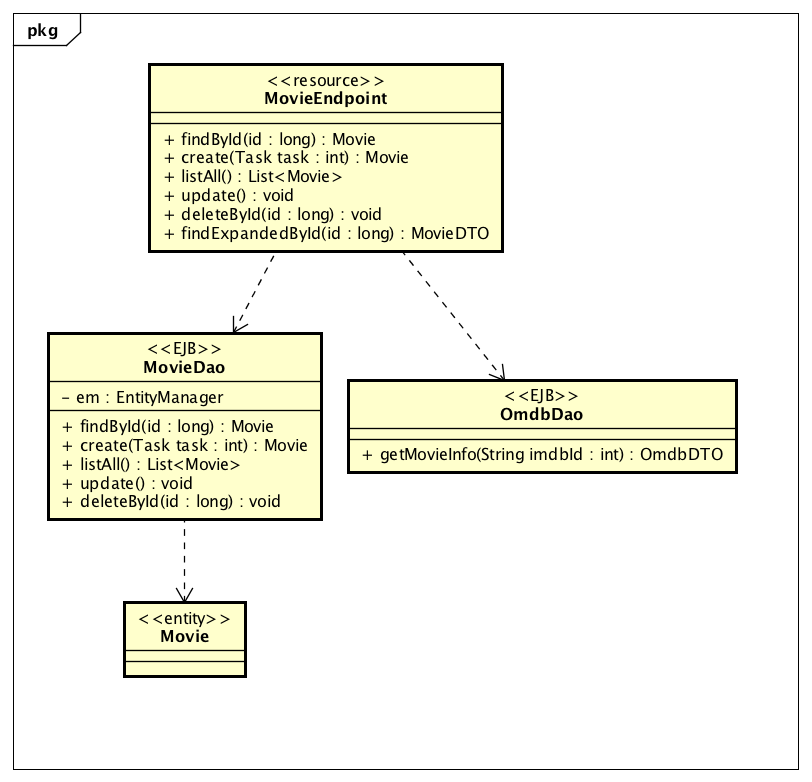
\includegraphics[width=\linewidth]{Images/democlass}
\end{figure}
\end{column}
\end{columns}
\end{frame}

\begin{frame}{Payara Micro - Micro Java EE}
\footnotesize MicroProfile: JAX-RS, CDI (Por servicio), Config, Fault Tolerance, Metrics\\
Implementación: EJB, JTA (Por servicio)\\
Por hacer: Location, Deployment, Orchestation, Balancing, Consistency, Patterns
\begin{figure}
\centering
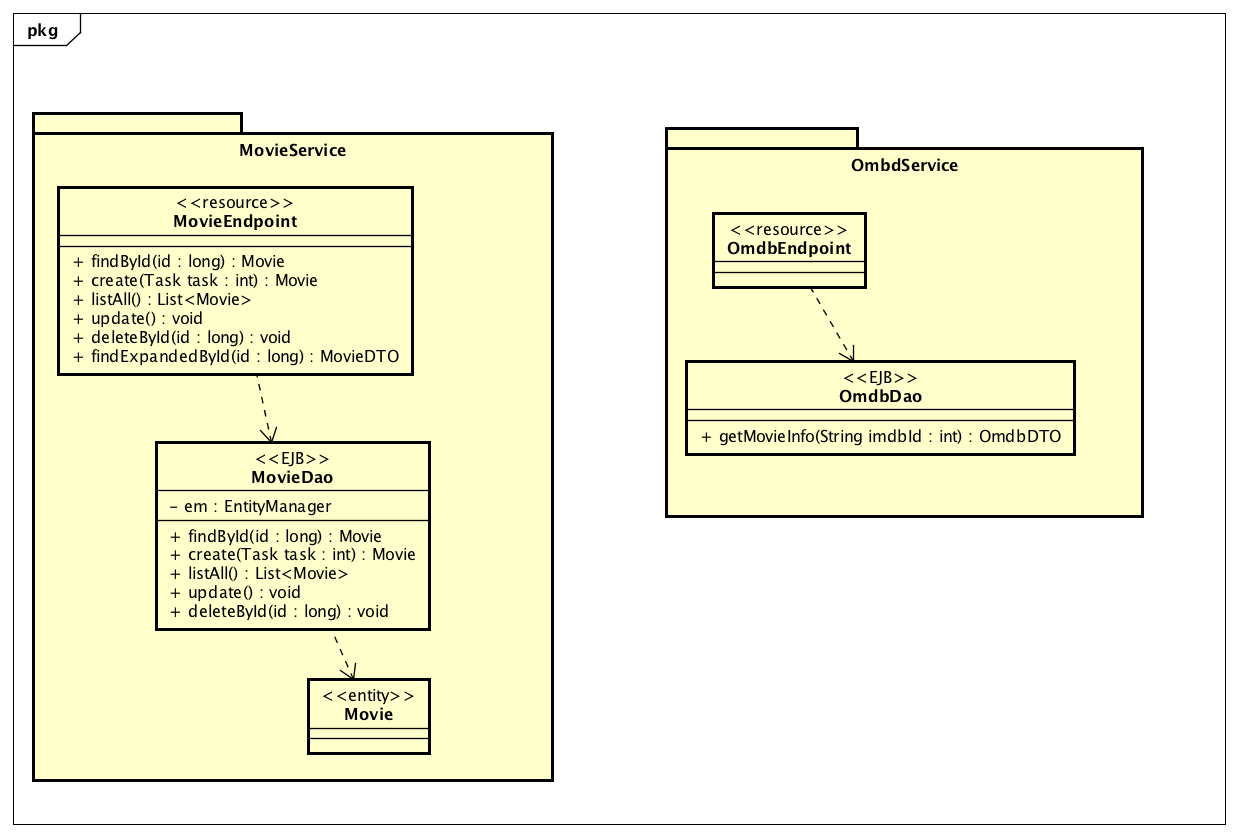
\includegraphics[width=0.95\linewidth]{Images/demomicro}
\end{figure}

\end{frame}

\begin{frame}[fragile]{Config}
\begin{lstlisting}
@Inject
@ConfigProperty(name = "omdbservice.url")
String omdbDaemonServiceUrl;
\end{lstlisting}
\end{frame}

\begin{frame}{Fault tolerance}

\begin{itemize}
\item Circuit Breaker
\item Bulkhead
\item Fallback
\item Retry
\item Timeout
\end{itemize}

\end{frame}


\begin{frame}[fragile]{Fault tolerance - Fallback, Timeout}
\begin{lstlisting}
@GET
@Path("/{id:[a-z]*[0-9][0-9]*}")
@Fallback(fallbackMethod = "findByIdFallBack")
@Timeout(TIMEOUT)
public Response findById(@PathParam("id") 
final String imdbId) {
...
}

public Response findByIdFallBack(@PathParam("id") 
final String imdbId) {
...
}
\end{lstlisting}
\end{frame}


\begin{frame}{Metrics}

\begin{itemize}
\item Vendor
\item Base
\item Application
\end{itemize}

\end{frame}

\begin{frame}[fragile]{Metric}
\begin{lstlisting}
@Inject
@Metric
Counter failedQueries;
\end{lstlisting}
\end{frame}

\begin{frame}{Gracias}
\begin{itemize}
\item me@vorozco.com
\item http://vorozco.com
\item http://github.com/tuxtor/slides
\end{itemize}
\begin{center}

\includegraphics[width=0.1\linewidth]{Images/cclogo}
\\
This work is licensed under a Creative Commons Attribution-ShareAlike 3.0 Guatemala License.
\end{center}
\end{frame}

\end{document}

